%%%%%%%%%%%%%%%%%%%%%%%%%%%%%%%%%%%%%%%%%%%%%%%%%%%%%%%%%%%
%                                                         %
%       This is documentation for the IFJ project.        %
%                                                         %
%%%%%%%%%%%%%%%%%%%%%%%%%%%%%%%%%%%%%%%%%%%%%%%%%%%%%%%%%%%


%------------------------------------------------%
%	    CONFIGURATION + IMPORTED PACKAGES        %
%------------------------------------------------%
\documentclass[10pt,a4paper,titlepage]{article}
\usepackage[english]{babel}
\usepackage[utf8]{inputenc}
\usepackage[margin=100pt]{geometry}


\usepackage{graphicx}   % Import pictures
\usepackage{ragged2e}   % fullfill paragraphs
\usepackage{multicol}

\begin{document}
%-----------------------------------------%
%	            TITLE PAGE                %
%-----------------------------------------%
\begin{titlepage}

\begin{center}
% Headings
\textsc{\LARGE Brno University of technology}\\[0.5cm]
\textsc{\large Faculty of Information Technology}\\[7cm]

% Title - lines
{ \huge \bfseries IFJ project}\\[0.3cm]
{ \Large \bfseries documentation}\\[0.5cm]
{ \bfseries team 034 variant II.}\\[1cm]

% authors
\begin{tabular}{  l | r | c }
  {\bf Martin Benes} & xbenes49 & 34 \\
  Ksenia Bolshakova  & xbolsh00 & 33 \\
  Petr Kratochvil    & xkrato47 & 0  \\
  Ondrej Polansky    & xpolan07 & 33 \\
\end{tabular}
\\[4cm]
% extensions
Extensions: \\
BASE \\
UNARY
\end{center}

\end{titlepage}
\newpage

%-----------------------------------------%
%	            CHAPTERS                  %
%-----------------------------------------%

\setcounter{page}{1}
\pagenumbering{arabic}

\section{Lexical analysis}

\begin{justify}
We did the scanner in two ways: singlethread and multithread work. Both variants work on the basis of a state machine.
The state machine was created on a basis of regular expression designs for each type of phrasems:
integer, real number (decimal point, positive or negative exponent), string, operator, identifier, keyword, comment.

The multithread scanner implementation used separate thread, read bytes from input, generates tokens and pushes
them to the queue. The parser then reads from the queue and processess the tokens in it. At some moment of multithread
implementing, we have come to the decision, that the singlethread scanner would be better, since we have got one member off.

\begin{center}
  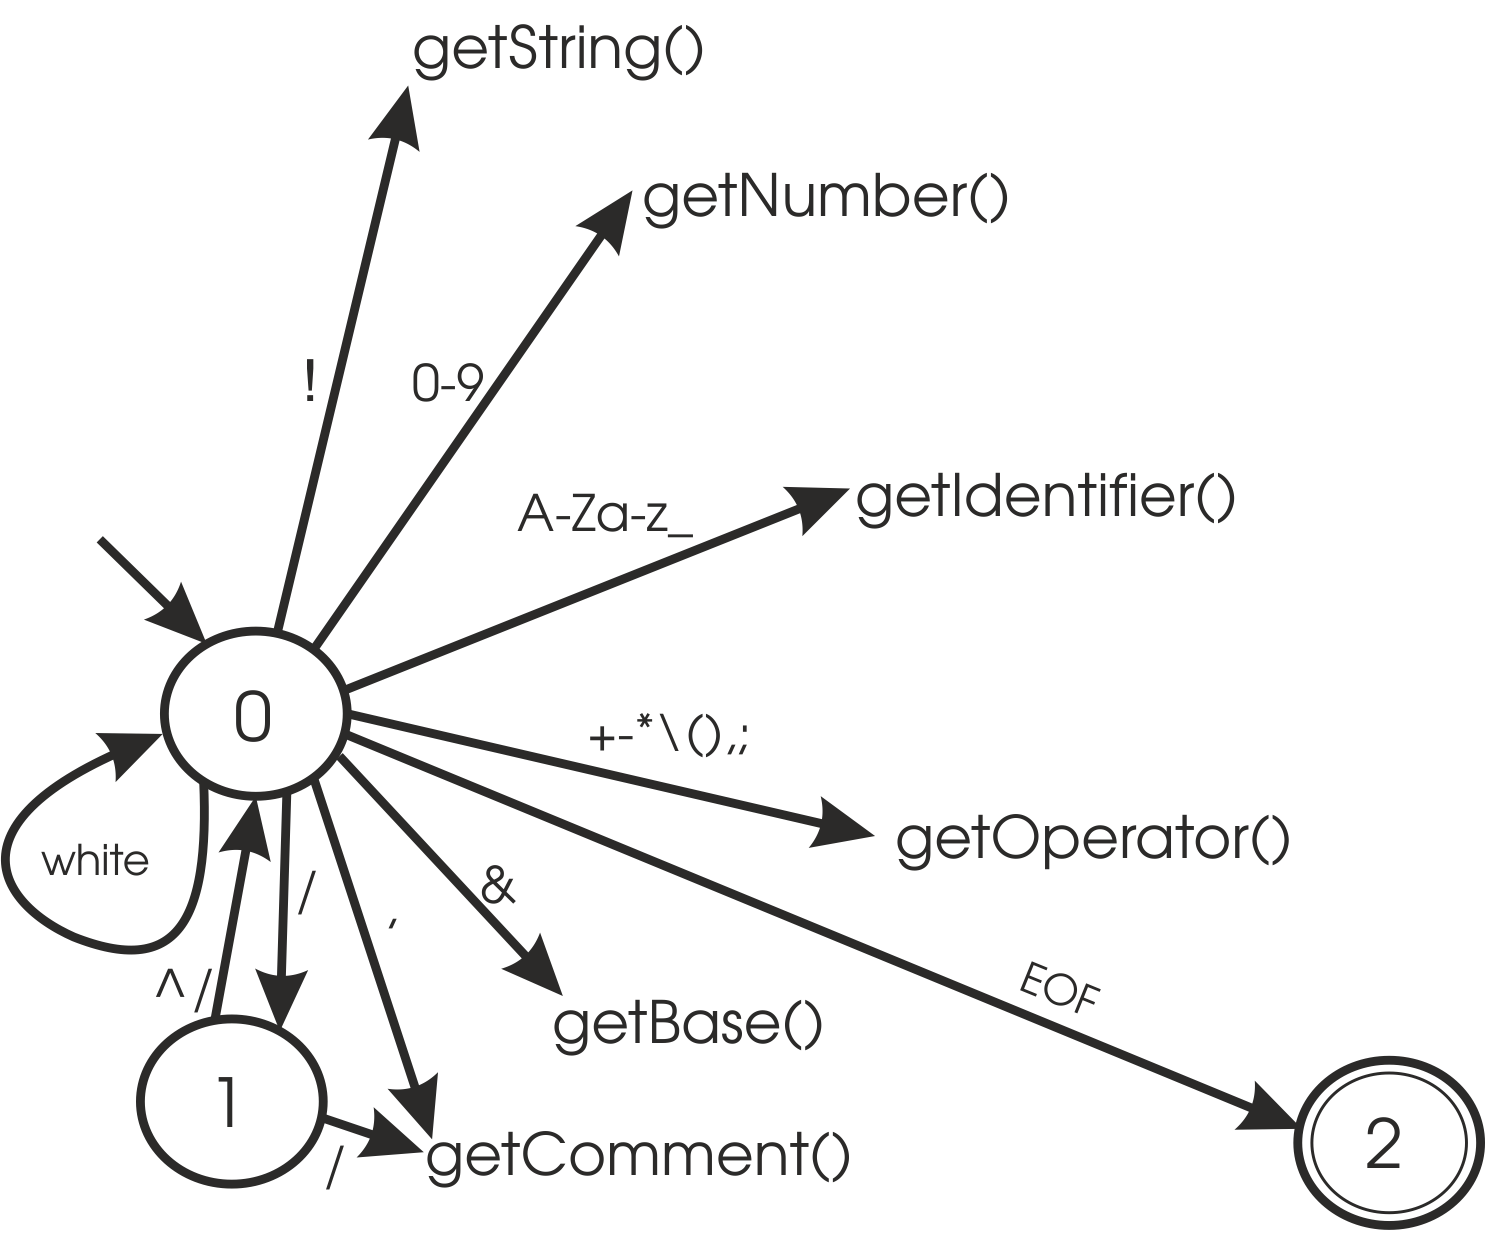
\includegraphics[width=0.35\textwidth]{img/general.png}
\end{center}

For the purpose of decomposition, the structure of the lexical analyzer was divided into several subprograms
that implemented individual parts.
\end{justify}

%%%%% getNumber %%%%%
\begin{justify}
Numbers, decimal and exponential numbers are scanned in the function \textit{getNumber()}.
\end{justify}
\begin{center}
  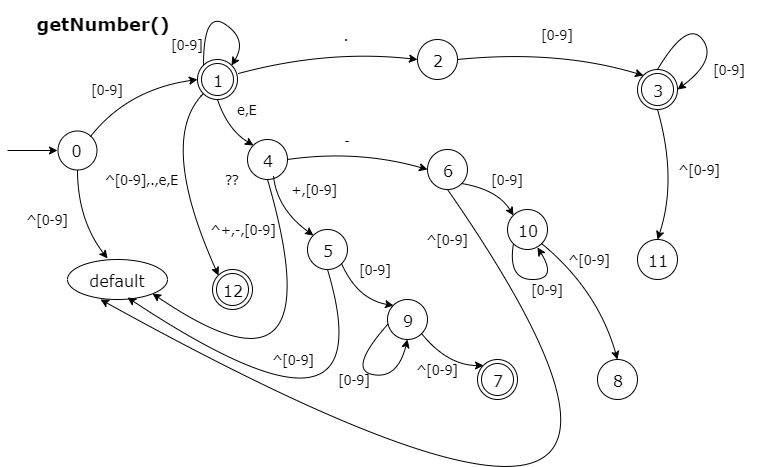
\includegraphics[width=0.45\textwidth]{img/getNumber.png}
\end{center}

%%%%% getString %%%%%
\begin{justify}
Strings are scanned in the function \textit{getString()}.
\end{justify}
\begin{center}
  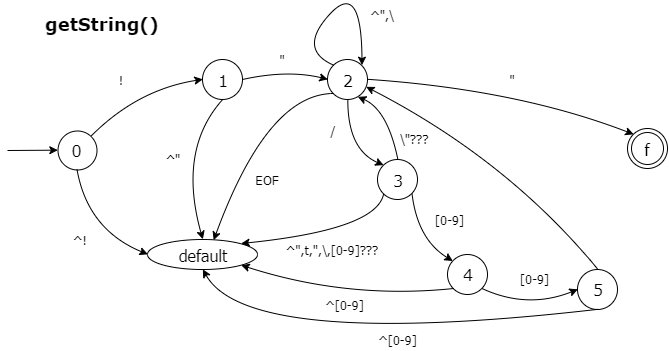
\includegraphics[width=0.4\textwidth]{img/getString.png}
\end{center}

%%%%% getComment %%%%%
\begin{justify}
The comments are scanned in the function \textit{getComment()}. We have simplified the "//" with "\textasciitilde".
\end{justify}
\begin{center}
  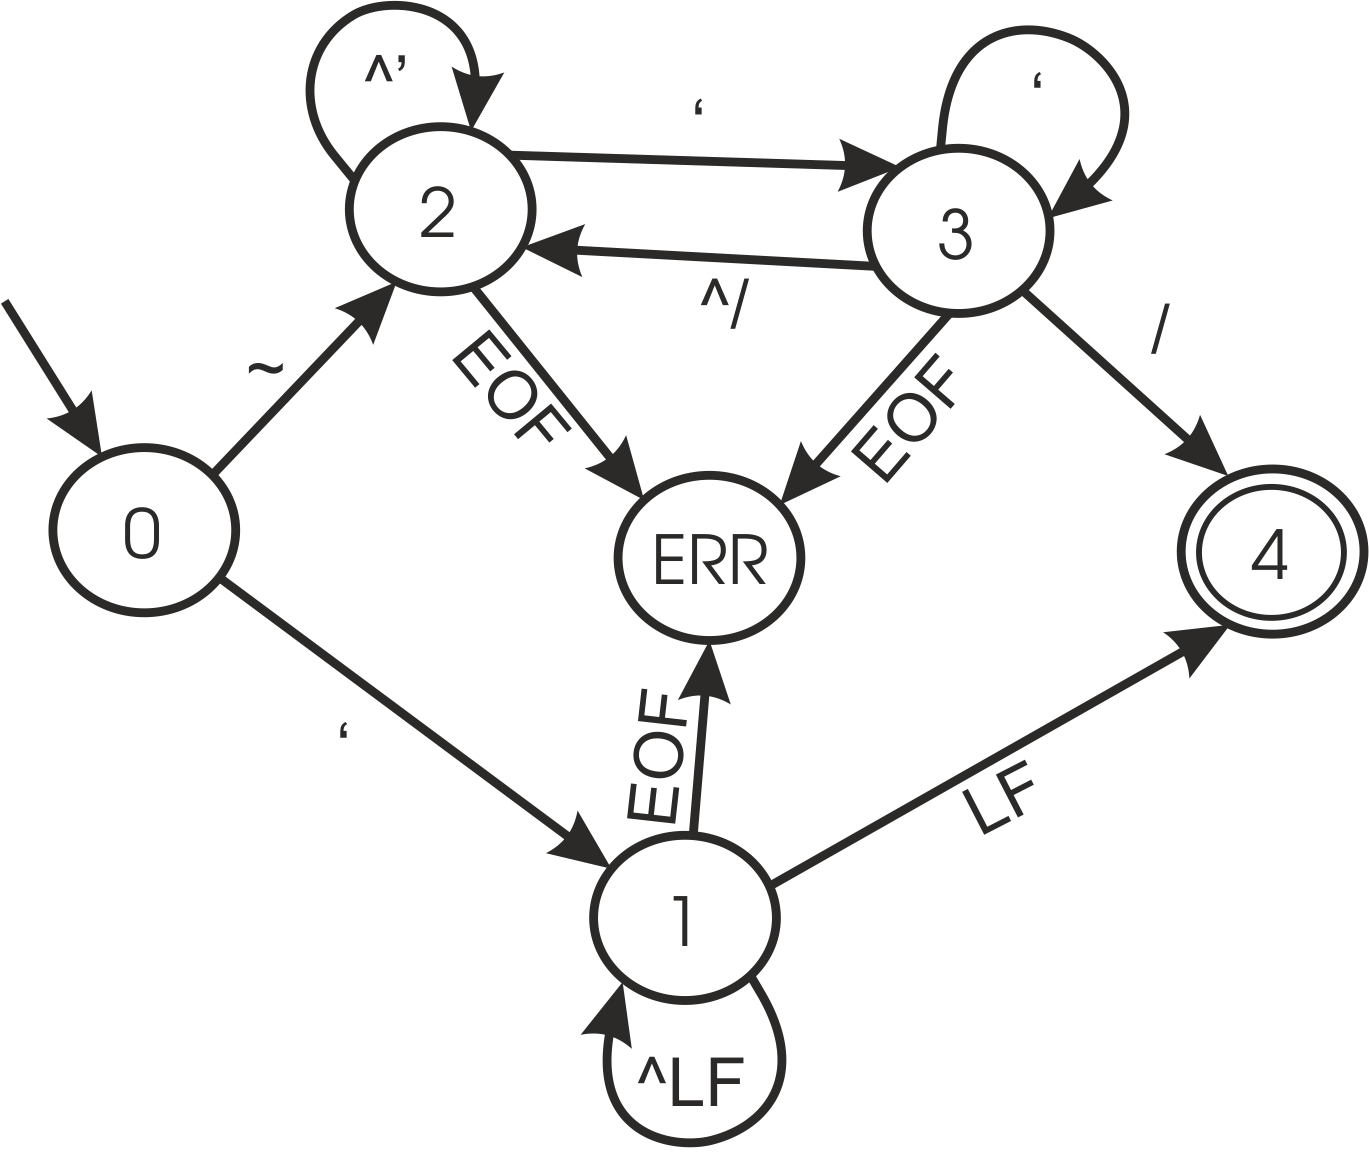
\includegraphics[width=0.4\textwidth]{img/getComment.png}
\end{center}

%%%%% getIdentifier %%%%%
\begin{justify}
Identifiers and keywords are scanned in the function \textit{getIdentifier()}.
\end{justify}
\begin{center}
  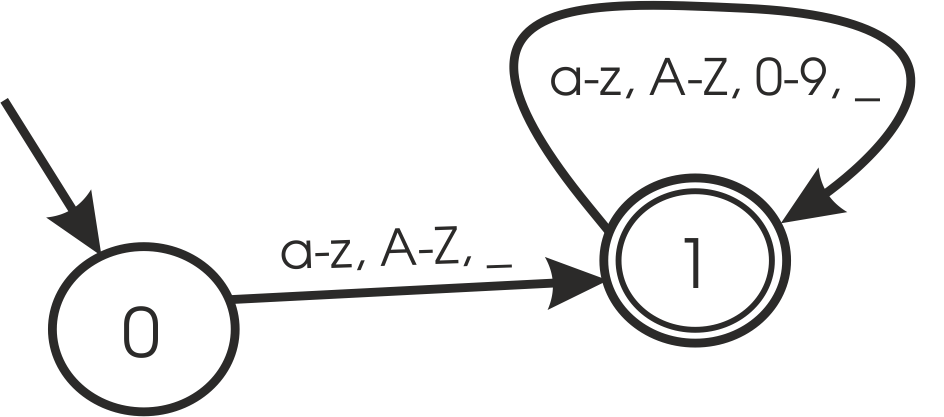
\includegraphics[width=0.35\textwidth]{img/getIdentifier.png}
\end{center}

%%%%% getOperator %%%%%
\begin{justify}
Operators are scanned in the function \textit{getOperator()}
\end{justify}
\begin{center}
  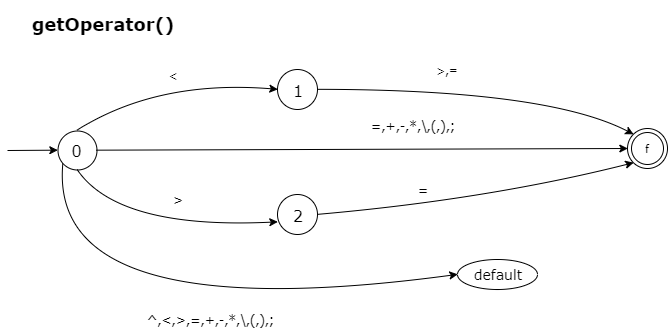
\includegraphics[width=0.35\textwidth]{img/getOperator.png}
\end{center}

\begin{justify}

To simplify the implementation, we use a wrapper modul \textit{io.h} to
be able to return bytes back to the input with the function \textit{returnByte()}.
\end{justify}

\newpage
\section{Tables}
\subsection{Table of constants}

\begin{justify}

The table contains all the important informations about symbols – variables and
functions. For the variables, it is a type and a name, for functions, it is a name,
a type of a return value, a list of parameters, a list of variables and an
indication, whether the function was defined.

Since the request was to use hash tables, we have a hash table of
functions and for each function, there is, among other things, a hash table of
variables. Hashing is performed by a hash function, as a key a name of the
function or the variable is used. In case of collision there is a rehash
function, which is based on linear probing and increases the index value
by three. This prevents clustering of entities when names (and therefore
fabricated indexes) are similar. The size of the table is set to a value
that cannot be divided by three so that the algorithm works all the time.

There is a starting size for each hash table and all hash tables resize
automatically when a half of the table is full. It typically doubles the size,
which might seem a little bit wasteful but it means there will not be that many
collisions and therefore the program will be faster. We do not expect that the
number of functions or variables in each function will be higher than a few
thousand so tables should not take too much space. During the operation of
resizing, every entity of the former table is rehashed and saved into a bigger
table.

The table of symbols is implemented in a file named symtable.c and the
interface is present in symtable.h. Table of symbols offers basic functions
for storing, modifying and reading all information about the symbols.

\end{justify}

\subsection{Other tables}

\begin{justify}

Many other tables are present in the program. Tables of keywords and operators
are simple arrays with linearly searching algorithm. Table of constants is
also an array with linear search algorithm but this table can actually
be resized by adding thirty to the current table size, since we expect only a
few constants. All other tables are implemented in tables.c and interface
is in tables.h.

\end{justify}


\begin{multicols}{2}
  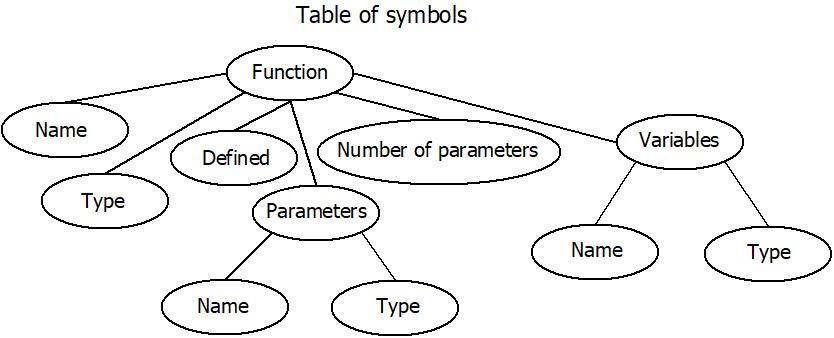
\includegraphics[width=0.4\textwidth]{img/TableOfSymbols.jpg}
  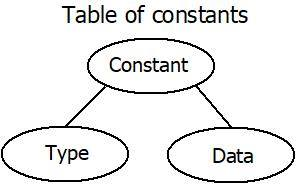
\includegraphics[width=0.3\textwidth]{img/TableOfConstans.jpg}
\end{multicols}

\newpage
% ------------------------------------------------------- %

\section{Syntactic analysis}

\begin{justify}
For the parser, we have decided to implement our LL-grammar design as
recursive descent. The main advantages are significant decomposition,
transparency of the code, as same as simplicity of extension of the
functionality etc. It requires a bit more abstract point of view on the
designed model during the implementation, nevertheless the draft is still
clear to see.
\end{justify}

% LL table
{\scriptsize
%{\footnotesize
  \begin{center}
    \begin{tabular}{ | l | c  c  l | } \hline
      1  & $<$GlobalBlock$>$              & $\rightarrow$ & $<$FunctionDeclaration$>$ $<$GlobalBlock$>$ \\ \hline
      2  & $<$GlobalBlock$>$              & $\rightarrow$ & $<$FunctionDefinition$>$ $<$GlobalBlock$>$ \\ \hline
      3  & $<$GlobalBlock$>$              & $\rightarrow$ & $<$Scope$>$ $<$GlobalBlock$>$ \\ \hline
      4  & $<$GlobalBlock$>$              & $\rightarrow$ & $\varepsilon$ \\ \hline
      5  & $<$FunctionDeclaration$>$      & $\rightarrow$ & {\it declare} $<$FunctionHeader$>$ \\ \hline
      6  & $<$FunctionDefinition$>$       & $\rightarrow$ & $<$FunctionHeader$>$ $<$Block$>$ $<$EndFunction$>$ \\ \hline
      7  & $<$FunctionHeader$>$           & $\rightarrow$ & {\it function} $<$FSymbol$>$ {\it (} $<$Parameters$>$ {\it )} {\it as} $<$DataType$>$ {\it \$} \\ \hline
      8  & $<$Scope$>$                    & $\rightarrow$ & {\it scope} {\it \$} $<$Block$>$ $<$EndScope$>$ \\ \hline
      9  & $<$FSymbol$>$                  & $\rightarrow$ & {\it id} \\ \hline
      10 & $<$VSymbol$>$                  & $\rightarrow$ & {\it id} \\ \hline
      11 & $<$DataType$>$                 & $\rightarrow$ & {\it string} \\ \hline
      12 & $<$DataType$>$                 & $\rightarrow$ & {\it double} \\ \hline
      13 & $<$DataType$>$                 & $\rightarrow$ & {\it integer} \\ \hline
      14 & $<$EndFunction$>$              & $\rightarrow$ & {\it end} {\it function} {\it \$} \\ \hline
      15 & $<$EndScope$>$                 & $\rightarrow$ & {\it end} {\it scope} {\it \$} \\ \hline
      16 & $<$Parameters$>$               & $\rightarrow$ & $<$VSymbol$>$ {\it as} $<$DataType$>$ $<$MoreParameters$>$ \\ \hline
      17 & $<$Parameters$>$               & $\rightarrow$ & $\varepsilon$ \\ \hline
      18 & $<$MoreParameters$>$           & $\rightarrow$ & {\it ,} $<$Parameters$>$ \\ \hline
      19 & $<$MoreParameters$>$           & $\rightarrow$ & $\varepsilon$ \\ \hline
      20 & $<$Block$>$                    & $\rightarrow$ & $<$VariableDefinition$>$ $<$Block$>$ \\ \hline
      21 & $<$Block$>$                    & $\rightarrow$ & $<$Assignment$>$ $<$Block$>$ \\ \hline
      22 & $<$Block$>$                    & $\rightarrow$ & $<$Input$>$ $<$Block$>$ \\ \hline
      23 & $<$Block$>$                    & $\rightarrow$ & $<$Print$>$ $<$Block$>$ \\ \hline
      24 & $<$Block$>$                    & $\rightarrow$ & $<$Condition$>$ $<$Block$>$ \\ \hline
      25 & $<$Block$>$                    & $\rightarrow$ & $<$Cycle$>$ $<$Block$>$ \\ \hline
      26 & $<$Block$>$                    & $\rightarrow$ & $<$Return$>$ $<$Block$>$ \\ \hline
      27 & $<$VariableDefinition$>$       & $\rightarrow$ & {\it dim} $<$VSymbol$>$ {\it as} $<$DataType$>$ $<$VariableInitialization$>$ {\it \$} \\ \hline
      28 & $<$VariableInitialization$>$   & $\rightarrow$ & {\it =} $<$Expression$>$ {\it \$} \\ \hline
      29 & $<$VariableInitialization$>$   & $\rightarrow$ & $\varepsilon$ \\ \hline
      30 & $<$Assignment$>$               & $\rightarrow$ & $<$VSymbol$>$ {\it =} $<$AssignmentValue$>$ {\it \$} \\ \hline
      31 & $<$AssignmentValue$>$          & $\rightarrow$ & $<$Expression$>$ \\ \hline
      32 & $<$AssignmentValue$>$          & $\rightarrow$ & $<$FunctionCall$>$ \\ \hline
      33 & $<$FunctionCall$>$             & $\rightarrow$ & $<$FSymbol$>$ {\it (} $<$Arguments$>$ {\it )} {\it \$} \\ \hline
      34 & $<$Arguments$>$                & $\rightarrow$ & $<$Expression$>$ $<$MoreArguments$>$ \\ \hline
      35 & $<$Arguments$>$                & $\rightarrow$ & $\varepsilon$ \\ \hline
      36 & $<$MoreArguments$>$            & $\rightarrow$ & {\it ,} $<$Arguments$>$ \\ \hline
      37 & $<$MoreArguments$>$            & $\rightarrow$ & $\varepsilon$ \\ \hline
      38 & $<$Input$>$                    & $\rightarrow$ & {\it input} $<$VSymbol$>$ {\it \$} \\ \hline
      39 & $<$Print$>$                    & $\rightarrow$ & {\it print} $<$Expression$>$ {\it ;} $<$PrintParameters$>$ {\it \$} \\ \hline
      40 & $<$PrintParameters$>$          & $\rightarrow$ & $<$Expression$>$ {\it ;} $<$PrintParameters$>$ \\ \hline
      41 & $<$PrintParameters$>$          & $\rightarrow$ & $\varepsilon$ \\ \hline
      42 & $<$Condition$>$                & $\rightarrow$ & {\it if} $<$Logic$>$ {\it then} {\it \$} $<$Block$>$ {\it else} {\it \$} $<$Block$>$ $<$EndIf$>$ \\ \hline
      43 & $<$Logic$>$                    & $\rightarrow$ & $<$Expression$>$ $<$ComparisonOperator$>$ $<$Expression$>$ \\ \hline
      44 & $<$ComparisonOperator$>$       & $\rightarrow$ & {\it $<$} \\ \hline
      45 & $<$ComparisonOperator$>$       & $\rightarrow$ & {\it $<=$} \\ \hline
      46 & $<$ComparisonOperator$>$       & $\rightarrow$ & {\it $>$} \\ \hline
      47 & $<$ComparisonOperator$>$       & $\rightarrow$ & {\it $>=$} \\ \hline
      48 & $<$ComparisonOperator$>$       & $\rightarrow$ & {\it $=$} \\ \hline
      49 & $<$ComparisonOperator$>$       & $\rightarrow$ & {\it $<>$} \\ \hline
      50 & $<$EndIf$>$                    & $\rightarrow$ & {\it end} {\it if} {\it \$} \\ \hline
      51 & $<$Cycle$>$                    & $\rightarrow$ & {\it do} {\it while} $<$Logic$>$ {\it \$} $<$Block$>$ $<$EndCycle$>$ \\ \hline
      52 & $<$EndCycle$>$                 & $\rightarrow$ & {\it loop} {\it \$} \\ \hline
      53 & $<$Return$>$                   & $\rightarrow$ & {\it return} $<$Expression$>$ {\it \$} \\ \hline
      54 & $<$Expression$>$               & $\rightarrow$ & {\bf calling ExpressionParse...} \\ \hline
    \end{tabular}
  \end{center}
}

\begin{justify}
The parser gains tokens from the scanner and calls the functions to process
the tokens (syntactically, call the semantic check in pedant, generate code
in generator). The functions expect the exact sequence of tokens of the exact
type, however if it will not acquire the right ones, the error is raised. This
process is similar to the designed one, it does not include the direct
implementation of the stack for the pushdown automaton though.
\end{justify}

\subsection {Expression parsing}
\begin{justify}
When the numeric expression is expected (arguments in function call, right
side of assignment), the separate predictive parser (ExpressionParse) is
called. The result is a stack, saved in semantic analyzer (pedant).

Logical expression (in the condition, or cycle) is understood as two
expressions separated with a comparison sign.

The scanner labels the identifiers of functions and variables as general
symbols. It is then retyped, based on the context in the parser.
\end{justify}

\section{Semantic analysis}
\begin{justify}
After the predictive parser processes the expression, it is saved in the
pedant as pre-fixed stack. At the end of the creation, predictive parser turns
the stack upside down, and checks the type compatibility. If it is needed,
the special tokens are inserted after the operand which needs to be converted.
In case of incompatibility, it raises error. It is then left behind in the
pedant.

Afterwards, the parser is accepted to proceed and it sends the target datatype,
expression has to be casted to. The stack is then generated, the possible
conversion afterwards, and the target to assign to.

For the logical comparison, the last type has to be memorized. When the
second stack will come, the typecast is send to convert the first, or the
second and typecast to the second one, or none of it.
\end{justify}

\section{Generator}
\begin{justify}
Generator possesses a state stack (GState stack) and a label stack.
When it handles stack from pedant or single token from pedant or parser,
the top of the state stack indicates, what to do with it.

The state stack is operated directly from the parser, which calls functions
G\_*, that pushes the state onto the stack, or directly generates some code,
or both. The result is, that the generator knows what to do, when it receives
a stack or a token is send, and generates correctly.

When a block (function, condition, loop) appears, the comparison and jumps
are generated and for that, unique name generator is essential. Our compiler,
generating label names 7 characters long, is limited to 56,8 billion of jumps,
names are in format \$aaaaaa, which appears as sufficient. The label name
is also pushed to the special label stack.

Later, when the block ends, the additional instructions, such as labels
and jumps are needed, so the function G\_EndBlock() is called. The generator
then finds what to end in the GState stack, and gains the right data from
label stack to insert the label name to the instruction.

Printing is, due to absence of instruction, that would print the top of the
stack, also provided by generating of new temporary frame (to avoid the
duplicity of the name when printing in cycle), creating a variable to it,
and print the variable.

When a declared, but not defined function is called, the parameter names
are not known to assign the arguments to in the function call. It is
replaced with $*<order>$ and moved in the function body. It also sets the
limit to the 999 parameters in single function.
\end{justify}
\newpage
% ------------------------------------------------------- %

\section{The split of work}
\subparagraph{Martin} (xbenes49) the parser, the generator
\subparagraph{Ksenia} (xbolsh00) the scanner, the expression generator and the documentation
\subparagraph{Petr} (xkrato47) {\it did not cooperate}
\subparagraph{Ondrej} (xpolan07) the tables (symbol, ...), ExpressionParse (syntax and semantic)

\end{document}


\section{The split of work}
\subparagraph{Martin} (xbenes49) the parser, the generator
\subparagraph{Ksenia} (xbolsh00) the scanner, the expression generator and the documentation
\subparagraph{Petr} (xkrato47) {\it did not cooperate}
\subparagraph{Ondrej} (xpolan07) the tables (symbol, ...), ExpressionParse (syntax and semantic)

\end{document}
